\documentclass{article}
\usepackage[utf8]{inputenc}
\usepackage{graphicx} %package to manage images
\usepackage{wrapfig}
\usepackage{multicol}
\usepackage[margin=0.1in]{geometry}
\title{301 Cheat Sheet}
\author{Tracy Nguyen, Renae Taylor and Are Oelsner}
\date{September 2017}

\begin{document}

\textbf{1. Introduction}\\ 
Compiler $\rightarrow$ Assembler (assembly language) $\rightarrow$ Machine
language $\rightarrow$ Hardware \\
System Components: Processor (datapath and control), Memory, I/O \\
Datapath- performs arithmetic operations \\
Control- commands datapath, memory, I/O devices \\
Operating System- interfaces between a user's program and the hardware; provides
a variety of services and supervisory functions by managing the resources of a
computer (handles basic I/O operations, allocates storage/memory, provides for
protected sharing of computer among multiple applications using it
simultaneously)\\
Volatile memory loses data when power off (DRAM/SRAM- main memory) //
Nonvolatile memory: magnetic disk, flash memory, optical disk; secondary memory.
\\
Networks: provides communication, resource sharing, and non-local access \\
Local area network (LAN) : Ethernet within a building, wide area network (WAN) :
the internet, wireless network: Wifi, Bluetooth.\\
\textbf{Instruction set architecture}: the hardware/software interface.
Specifies the instructions that the architecture understands. Classified by
number of addresses included in instruction. \\
Different addressing architectures: 0 address architecture (stack: operations
take operands from top of stack, then push result onto stack), 1 address
architecture (assume one operand in accumulator, specify other address), 3
address architecture (MIPS).\\
Immediate addressing: data appears in constant part of instructions, register
addressing: data is in register specified in instruction. \\
CISC vs. RISC: RISC makes hardware design simpler (doesn't guarantee increased
speed!); CISC makes hardware like software- easier compilation, and optimizes
program size.\\

\textbf{2. Power and Performance}\\
\underline{Response/Execution Time}- total time required to complete a task
(start - end time); includes everything (disk/memory accesses, I/O, OS
overhead); determines system performance, measured in sec \\
\underline{Throughput/Bandwidth}- total amount of work done in given time\\
\underline{CPU Time}- actual time spent executing code for specific task
(doesn't include I/O or time-sharing); comprises user CPU time (in program) and
system CPU time (in OS performing tasks on behalf of program) \\
\underline{Clock Cycle}- determines when events take place and runs at constant
rate; Clock Rate = 1 / Clock Cycle $\rightarrow$ 500 MHz = 1/2ns; 1 ns =
$10^{-9}$s\\
$\rightarrow$ Clock Period: duration of clock cycle (250 ps = 0.25 ns =
$250\times10^{-12}$s \\
$\rightarrow$ Clock Frequency/Rate: cycles per second (4.0 GHz = 4000 MHz =
$4.0\times10^{9}$Hz or cycles/sec) \\
\underline{Instruction Count}- determined by program, ISA, and compiler \\
\underline{Clock Cycles Per Instruction}- determined by hardware, CPI is average
of all instructions executed in program \\
\underline{Performance Affected By}: Algorithms (affects IC, possibly CPI),
Programming Language (IC, CPI), Compiler (IC, CPI), ISA (IC, CR, CPI) \\ \\
Execution Time:
$Performance_{x} = \frac{1}{Execution\ Time_{x}}$ \\ \\
Relative Execution Time ("X is n times faster than Y"):
$\frac{Performance_{x}}{Performance_{y}} = \frac{Execution\ Time_{y}}{Execution\
Time_{x}} = n$ \\ \\
CPU Time = CPU Clock Cycles x Clock Cycle Time = $\frac{CPU\ Clock\
Cycles}{Clock\ Rate}$ \\ \\
Clock Cycles = Instruction Count x Cycles per instruction \\
CPU Time = IC x CPI x Clock Cycle Time = $\frac{Instruction\ Count\ \times\
CPI}{Clock\ Rate}$ \\ 
Performance (instructions/sec) = Clock Rate / CPI \\ \\
The Big Picture: \\
CPU Time $= \frac{Instructions}{Program} \times \frac{Clock\
Cycles}{Instruction} \times \frac{Seconds}{Clock\ Cycles}$\\~\\
CPU Clock Cycles = $\sum_{i=1}^{n} (CPI_{i} \times C_{i})$ \\ \\
Weighted Average CPI: \\
CPI = $\frac{Clock\ Cycles}{Instruction\ Count}$ = $\sum_{i=1}^{n} (CPI_{i}
\times \frac{Instruction\ Count_{i}}{Instruction\ Count})$ \\~\\
Amdahl's Law: $Exec_{new} = Exec_{old} \times ((1-fraction_{enh}) +
\frac{fraction_{enh}}{Speedup_{enh}})$ \\~\\
Speedup = $\frac{Execution  \ time \ without \ enhancement}{Execution \ time \
with \ enhancement}$ \\~\\
Improving an aspect of computer e.g. clock cycles $\neq$ proportional
improvement in overall performance. \\
$T_{improved} = \frac{T_{affected}}{improvement \ factor} + T_{unaffected}$ \\


Execution time is the best performance measure. Power is limiting factor.
Multicore processors require parallel programming (hard to do). Tricks to
improve power: cooling device or turn off unused parts of chips in given clock
cycle. \\

$\textbf{3. MIPS Stuffs}$\\
Op types\\
%\begin{wrapfigure}{R}{0.3\textwidth}
%\includegraphics[do size stuff here]{optypes.jpg}]
%\caption{op types}
%\end{wrapfigure}
R-type: Register 
6 bit opcode 000000,
5 bit rs,
5 bit rt,
5 bit rd,
5 bit shamt,
6 bit funct \\
I-type: Data Transfer
6 bit opcode,
5 bit rs,
5 bit rt,
16 bit address/immediate \\
J-type:
6 bit opcode 00001X,
26 bit address \\
J-Type instructions are only j and jal
• I-Type is all instructions immediate
operand, branch instructions, and load
and store instructions
• R-Type is all arithmetic and logic with
all operands in registers, shift
instructions, and register direct jump
instructions (jalr and jr)  \\
MIPS Static Data Address: 0x10010000, MIPS Main: 0x400000 \\

Fetch-Execute Cycle: \\
1) Copy the word referred to by the program counter (PC) into the instruction
register (IR) [Fetch] \\
2) Incrememnt the address stored in the PC \\
3) Decode and execute the contents of the IR [Execute] \\
4) Unless a stop instruction, go back to step 1\\

  
  Need to store return address as well as any volatile registers you are using
  before calling a function that you haven't written. ".ent" and ".end" for
  functions. \\
  1's complement: negate binary number 

  $\textbf{2's complement}$ \\
  Leading zeroes means positive, leading 1s mean negative. To convert from
  positive to negative (or vice versa), invert every bit then add one.\\
  Converting from two’s complement to
  decimal: $(x_{31} \times - 2^{31})+ (x_{30}\times 2 ^{30})+... +(x_1 \times
  2^1) + (x_0 \times 2^0)$ where $x_i$ means the ith bit of x. \\
  Convert -72 to an 8-bit, twos complement binary number: 
  Convert the magnitude, 72 to binary. The easiest way is to convert it to hex
  first. 72/16 = 4 remainder 8, so 7210 = 4816 = 10010002. \\
  Pad to 8 bits: 01001000. Negate the number by inverting the bits and adding 1
  $\to$ 10111000.\\~\\
  Positive numbers have infinite number of preceding 0s, Negative numbers have
  infinite number of preceding 1s. \\
  Recursive Functions in MIPS: 1. Aquire storage for procedure variables. 2.
  Perform calculations in function. 3. Place result in place accessible to
  caller. 4. Return control to caller.\\
  \begin{multicols}{3}
Example for fact:\\
  addiu \$sp, \$sp, -8\\
  sw \$ra, 0(\$sp)\\
  sw \$a0, 4(\$sp)\\
  li \$t0, 1\\
  blt \$a0, \$t0, lessThan\\
  addi \$a0, \$a0, -1\\
  jal fact \\
  lw \$a0, 4(\$sp)\\
  mul \$v0, \$v0, \$a0\\
  lw \$ra, 0(\$sp)\\
  addiu \$sp, \$sp, 8\\
  jr \$ra \\~\\
  Another Example Recursive Function $\to$

    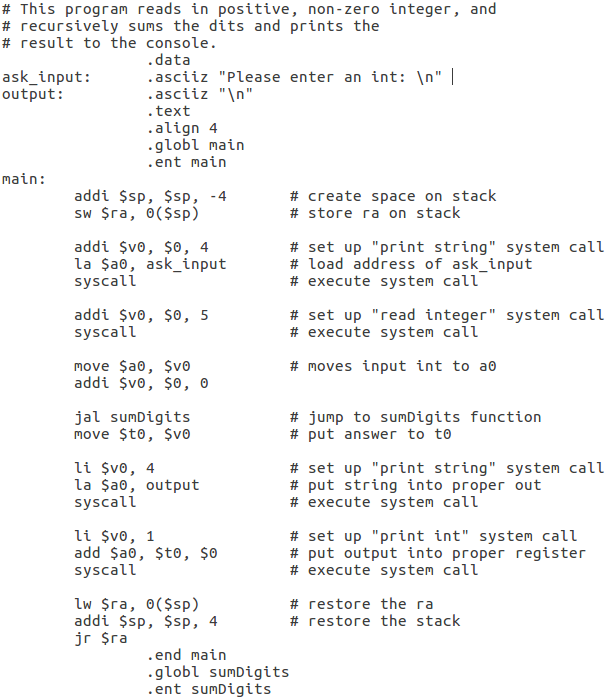
\includegraphics[width=60mm]{mipsrecursive1.png}
    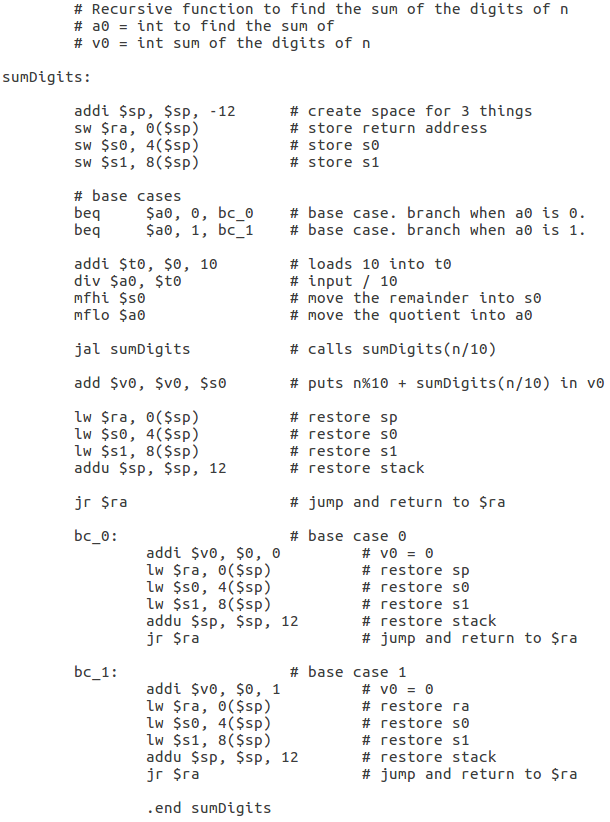
\includegraphics[width=50mm]{mipsrecursive2.png}

  \end{multicols}
  \$sp points to last item in stack, not next empty space. \\
  Hexadecimal: 0–9 to represent values zero to nine, and A,B,C,D,E,F to
  represent values ten to fifteen.\\
  Registers: \\
  R0: [r0], R1:  [at], R2:  [v0], R3:  [v1], R4:  [a0], R5:  [a1], R6:  [a2],
  R7:  [a3], R8:  [t0], R9:  [t1], R10: [t2], R11: [t3], R12: [t4], R13: [t5],
  R14: [t6], R15: [t7], R16: [s0], R17: [s1], R18: [s2], R19: [s3], R20: [s4],
  R21: [s5], R22: [s6], R23: [s7], R24: [t8], R25: [t9], R26: [k0], R27: [k1],
  R28: [gp], R29: [sp], R30: [s8], R31: [ra] \\
  Two types of add/sub instructions: 
  add/addi/sub - overflow causes exception,
  addu/addiu/subu - overflow does not cause exception, as unsigned integers are
  usually used for memory addresses. \\ 
  Woody Machine Language: \\
  CopyFrom 000,
  CopyTo 001,
  Add 010,
  Subtract 011,
  Read 100,
  Print 101,
  IfNegGoTo 110,
  Stop 111 \\
\end{document}

